%
\documentclass[10pt]{report}
\usepackage{hyperlatex}
\usepackage[dvips]{color}
\usepackage[dvips]{graphicx}
\usepackage{longtable}
\usepackage{makeidx}
\W\usepackage{sequential}
\xmlattributes{body}{bgcolor="#ffffe6"} 
\htmltitle{Verde Users Manual Version 2.6}
\htmladdress{support@elemtech.com}

\W\begin{iftex}
  \sloppy
  \topmargin .5in
  %\headsep 30pt
  \evensidemargin 0pt
  \oddsidemargin 0pt
  \textwidth 6.5in
  \textheight 8.5in
\W\end{iftex}          

\title{Verde Users Manual Version 2.6}
\author{Karl G. Merkley, Ray J. Meyers, Clint Stimpson, Corey Ernst}
\begin{document}

\maketitle
\W\begin{iftex}
  \pagenumbering{roman}
  \setcounter{page}{1}   
  \tableofcontents
  \listoffigures
  \listoftables
  \newpage
  \pagenumbering{arabic}
\W\end{iftex}

\chapter{Introduction}
\label{sec:introduction}

Verde (Verification of Discrete Elements) 
is a program designed to verify the properties of a finite element 
mesh stored in Exodus II format\cite{schoof}\cite{netCDF}.
Verde uses a variety of verification 
algorithms and graphics to thoroughly analyze the individual and combined properties 
of the mesh and to help the user detect any problems that may exist.  
Verde can be run in two modes.  The default mode provides a graphical 
user interface (GUI) and tools for visualizing the model and displaying 
problem areas of the mesh.   
The GUI was developed using Qt, the cross-platform C++ GUI 
toolkit \cite{trolltech}.
Verde can also be run from the command line in a batch 
mode.  It is designed for high throughput of large meshes.  It is  
easily extensible and built to allow the addition of new element types and 
metrics as they become available.


\section{Element Types}
\label{sec:element_types}

Verde will analyze the following element types:

\begin{center}
\begin{tabular}{lll}
Hexes     & Tetrahedra                 \\
Pyramids  & Wedges (triangular prisms) \\
Knives    & Quads                      \\
Triangles & Bars (beams)               \\
\end{tabular}
\end{center}


Verde will handle all higher-order variants of these types provided they 
are defined using the standard Exodus II node numbering; however, for 
higher-order elements, the metrics are calculated based on the linear 
versions of the elements.



\section{Types of Verification}
\label{sec:verification_types}

Verde 2.6 performs mesh verification in three areas:


\begin{enumerate}
\item
{
\textit{Individual Element Metrics}. The individual characteristics 
of each element are verified by calculating common metrics depending 
on the element type. Verde calculates one or more metrics for each element 
type supported.  For each metric, the minimum, maximum, average, and standard 
deviation of each metric are tracked, as well as the elements at which 
the minimum and maximum occur.  All elements whose metric values fall 
outside the user-definable acceptable range are flagged as failed. 
}
\item
{
\textit{Topology Checks.} The topology of the mesh is carefully 
analyzed, looking for any defects in the mesh connectivity or continuity 
that would invalidate the mesh.  Verde reports the number of exterior 
entities for the mesh, checks for manifold topology, and if the
object is manifold, calculates the 
Euler number and infers the probable overall topology.
In addition, it checks for adjoining
quadrilateral faces in the mesh that share only three nodes.
}
\item
{
\textit{Interface Checks.} The exterior surface of the mesh is 
carefully analyzed.  Exterior elements are checked for 
coincidence.  In this way, potential problems such as incorrect mesh 
joins and multiply-meshed regions can be detected.  
In batch mode, an optional output file can be created 
(in Exodus II format) which contains 
information from the analysis such as the exterior skin of the mesh, 
inferred model edges, and failed elements.  This file can be read by 
Verde in the interactive mode or other tools that read Exodus II data
to establish orientations and locations 
of bad elements and to explore and understand how to improve the current 
mesh.
}
\item
{
\textit{Quads Sharing Three Nodes.} Hexahedral elements and Quadrilateral elements
are checked to see if any faces of Hexahedral elements or Quadrilaterals share 
three nodes with another face of a Hexahedral element or Quadrilateral.
The check may optionally be performed on the exterior mesh, or on the entire mesh.
}
\end{enumerate}


\section{Invoking Verde}
\label{sec:invoking}

The Verde graphical user interface (GUI) can be invoked from the 
command prompt.


\begin{center}
\% verde [options] [journal\_file.jou] [input\_file.gen]
\end{center}


where the input file is the file to be verified (in Exodus II format) and the 
options are optional control flags.  Options are preceded by the ``-'' 
character (``minus'' or ``dash'') and can be specified in any order. 
Current valid options for version 2.6 are:
\begin{center}
\begin{tabular}{lp{4in}}
-help & Print this summary                                                   \\
-batch & Runs verde in batch mode                                            \\
-blocks $<$\$val$>$ & Specifies block(s) to be processed (e.g. 1,5-7,9)      \\
-individual & Prints metrics for each block individually                     \\
-defaults $<$\$val$>$ & Specifies path and file of defaults file (e.g ../defaults1) \\
-nodefaults & Do not process .verde default file                             \\
-nointerface & Suppresses mesh interface verification calculations           \\
-nometrics & Suppresses element metric calculations                          \\
-output $<$\$val$>$ & Generates an Exodus II output file specified by $val$  \\
-notopology & Suppresses mesh topology verification calculations             \\
-print\_failed\_elements & Prints individual failed elements and values      \\
-version & Prints the verde version number                                   \\
-quads\_share\_3\_nodes $<$\$val$>$ & Check entire mesh, exterior quads, 
or nothing for quads sharing 3 nodes (all, exterior, none)                   \\
\end{tabular}
\end{center}
If Verde is invoked without the optional file name, a blank screen is displayed and 
the user may select a file using the File/Open menu item.


The basic syntax of the Verde batch command is:

\begin{center}
\% verde --batch [options] [journal\_file.jou] input\_file.gen 
\end{center}

For more details regarding the batch execution of Verde, see 
section \ref{sec:batch},
\xlink{ Controlling Verde in Batch Mode}{verde_batch.html}.


\chapter{An Overview of the GUI}
\label{sec:overview}

The Verde GUI is composed of a menu bar, a tool bar, three dockable 
windows, and a graphics display area as shown in figure \ref{fig:blank}.

\htmlrule
\begin{figure}[htb]
  \begin{center}
    \texorhtml{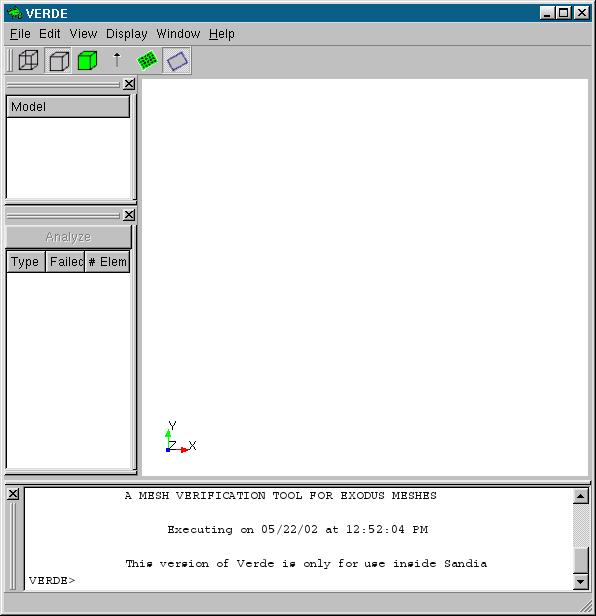
\includegraphics[height=3.8in]{images/blank_screen.eps}}
      {\htmlimage{images/blank_screen.jpg}}
    \caption{Verde Main Screen.}
    \label{fig:blank}
  \end{center}
\end{figure}     
\htmlrule


The menu bar includes functions for File operations 
such as loading a model, printing, saving an image file and exiting the 
program.  The Edit menu allows the user to specify 
parameters for the element metrics and user preferences.  The View menu 
controls the graphics viewing parameters.  The  
Display menu allows the user to control the graphics 
display of the model.  The Windows menu 
provides controls the visibility of the dockable windows. 
The Help menu provides access to this 
documentation.


The tool bar allows the user to specify the graphics 
display modes of the model as wire frame, hidden line, or shaded 
image.  It also provides options to toggle on the display of model normals,
surfaces, and edges.

There are three dockable windows.  The Model window controls the portions
of the model that are displayed.  The Results window controls the display
of verification results, and the Command line window allows command input
and is used to echo textual results.


\section{Controlling the Verde GUI}
\label{sec:controlling}


The following sections will give an explanation of each of the windows, 
menu items and dialog boxes in the Verde GUI.

\subsection{Model Window}
\label{model_window}

The Model Window is located in the 
upper left hand corner by default.  An example of this window is 
shown in figure \ref{fig:model_window}.  This window shows the current model 
that is loaded and a list of the blocks, node sets and side sets 
that are active and inactive in 
the model.  Right clicking on any element at the lowest level of the
tree structure will bring up a pop up menu that provides options for
activating or deactivating any given item.  Multiple items may be
selected using the shift or control keys.
When a block is inactive, the data 
for that block is not in memory.  It will not be displayed and no 
calculations will be performed on that block.  When a block is made 
active, the data for that block is read from the Exodus II file, the 
block is displayed and calculations can be performed.  Node set and
side set activation is independent of block activation.

\htmlrule
\begin{figure}[tbh]
  \begin{center}
    \texorhtml{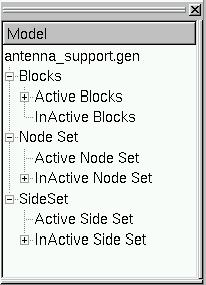
\includegraphics[width=2.0in]{images/model_window.eps}}
              {\htmlimage{images/model_window.jpg}}
    \caption{Verde Main Screen.}
    \label{fig:model_window}
  \end{center}
\end{figure}     
\htmlrule


\subsubsection{Node Set Display}
\label{nodesets}

Node sets are displayed as filled magenta squares drawn at each node where the
node set is applied as shown in figure \ref{fig:nodesets}. This display
is useful for verifying the correct application of nodal boundary conditions
in the model.

Node display sizes can be modified in the Edit/Preferences dialog as
described in section \ref{preferences}.

\htmlrule
\begin{figure}[tb]
  \begin{center}
    \texorhtml{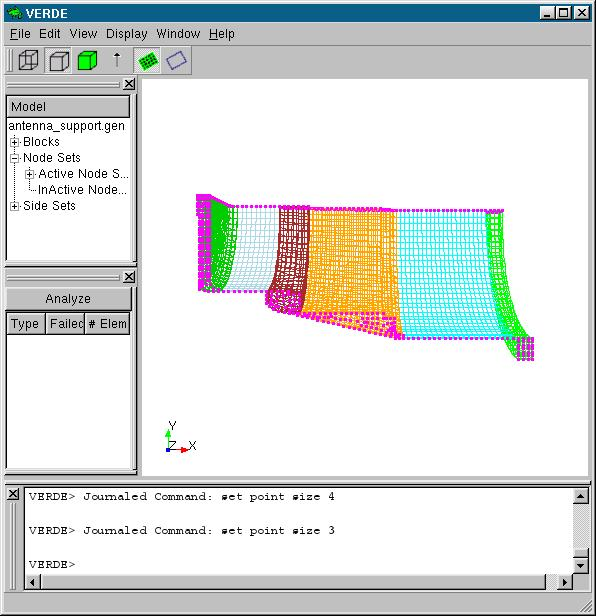
\includegraphics[height=3.8in]{images/nodesets.eps}}
              {\htmlimage{images/nodesets.jpg}}
    \caption{Node Set Display.}
    \label{fig:nodesets}
  \end{center}
\end{figure}     
\htmlrule

\subsubsection{Side Set Display}
\label{sidesets}

Side sets are displayed as magenta facets drawn on the face or edge of 
each element where the
side set is applied as shown in figure \ref{fig:sidesets}. The side set display
facets are slightly smaller than the faces of the elements that they are
drawn on.  This allows the user to verify that individual elements were not
skipped when the boundary condition was applied.

Side sets defined on the face of an element are only visible when viewed
from the side that they are defined on.  For example, shell elements may
have side sets placed on the forward or the reverse face.  A side set placed
on the forward face will not be visible when viewed from the reverse side
of the model.

\htmlrule
\begin{figure}[tbh]
  \begin{center}
    \texorhtml{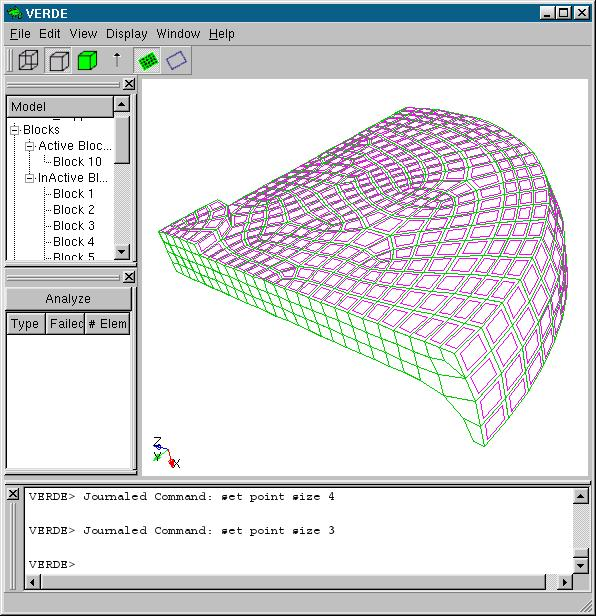
\includegraphics[height=3.8in]{images/sidesets.eps}}
              {\htmlimage{images/sidesets.jpg}}
    \caption{Side Set Display.}
    \label{fig:sidesets}
  \end{center}
\end{figure}     

\subsection{Results Window}
\label{results_window}
The Results Window is typically located below the Model Window.  
The Analyze button is located on this window and is inactive, as 
shown by its grayed out status, until a model is imported into Verde.  
After a successful analysis of the model, a list of 
element types, failure cases (metric, topological, and interface), 
and number of failed components is 
displayed in this window.  Selecting one of these rows causes the 
failed items to be highlighted on the graphics model.  Selecting
the highlighted item turns off the failed element display. The results 
of a metrics calculation is shown in figure \ref{fig:results_window}.

\htmlrule
\begin{figure}[tbh]
  \begin{center}
    \texorhtml{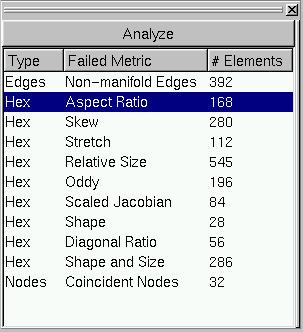
\includegraphics[width=2.0in]{images/results_window.eps}}
              {\htmlimage{images/results_window.jpg}}
    \caption{Results Window.}
    \label{fig:results_window}
  \end{center}
\end{figure}     


\subsection{Command Line Window}
\label{command_window}
The Command Line window is normally located along the bottom of the 
main Verde window.  This window allows the user to type in Verde 
commands.  It is also used to display the textual results of the 
calculate command as shown in figure \ref{fig:command_window}.

\htmlrule
\begin{figure}[tbh]
  \begin{center}
    \texorhtml{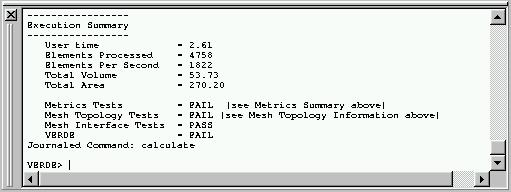
\includegraphics[width=4.0in]{images/command_window.eps}}
              {\htmlimage{images/command_window.jpg}}
    \caption{Command Line Window.}
    \label{fig:command_window}
  \end{center}
\end{figure}     

A user cannot execute all commands possible in the GUI
from the command line.  For example, there are no command line
options to rotate, translate or zoom the model.  However, most
commands are available in both modes.
A complete list of the command line options is given in Appendix C.

\subsection{File Menu}

The File menu provides standard file manipulation capabilities for 
loading an Exodus II file into Verde, reading and recording journal 
files and ending journal file recording, printing, capturing screen 
images, saving a model to Exodus II format,
\footnote %What do we do with this?
{
In this documentation file formats of Exodus II and Genesis are 
used interchangeably.
}
and exiting the program.


\subsubsection{Open Mesh}
\label{open_mesh}

If Verde is invoked without the optional file name, a blank screen is 
displayed and the user must select a model using the File/Open Mesh 
dialog as shown in figure \ref{fig:open_mesh}.

\htmlrule
\begin{figure}[tbh]
  \begin{center}
    \texorhtml{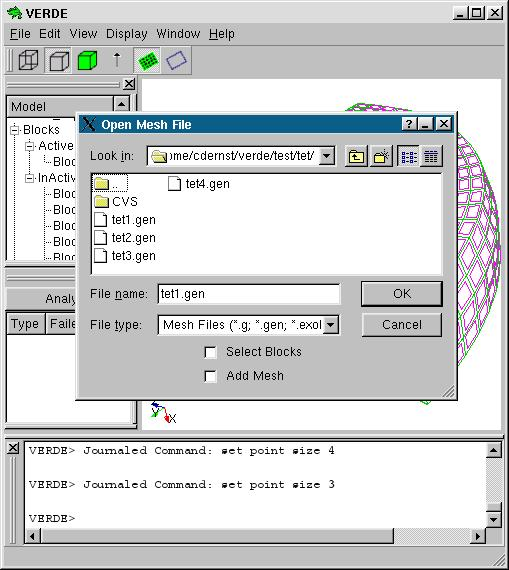
\includegraphics[height=3.8in]{images/file_open.eps}}
              {\htmlimage[hspace=3]{images/file_open.jpg}}
    \caption{Verde Open Mesh dialog.}
    \label{fig:open_mesh}
  \end{center}
\end{figure}     
\htmlrule

The Open Mesh dialog includes an option that allows the user to select 
blocks to be imported from the Exodus II file. The block 
selection dialog lists the blocks that are defined in the Exodus II file 
and the element type for each block. Verde considers the imported 
blocks ``active''.  Only active blocks are displayed in the graphics 
region and considered during metrics and topology calculations.

If there is an existing model in Verde 2.6, an additional checkbox
will appear labeled "Add Mesh."  This will allow additional models to
be added into the existing model.  When models are concatenated, the
original element and node ids are replaced with new global ids.

When the mesh has been imported, the skin of the model is displayed in 
the viewing region as shown in figure \ref{fig:model_screen}.

Verde always remembers the previous directory from which a file was 
selected and opens any subsequent file dialog boxes to this previous directory. 
If no previous directory exists, as when Verde is first invoked, the first file 
dialog defaults to the directory from which Verde is running, "./". 

\htmlrule
\begin{figure}[tbh]
  \begin{center}
    \texorhtml{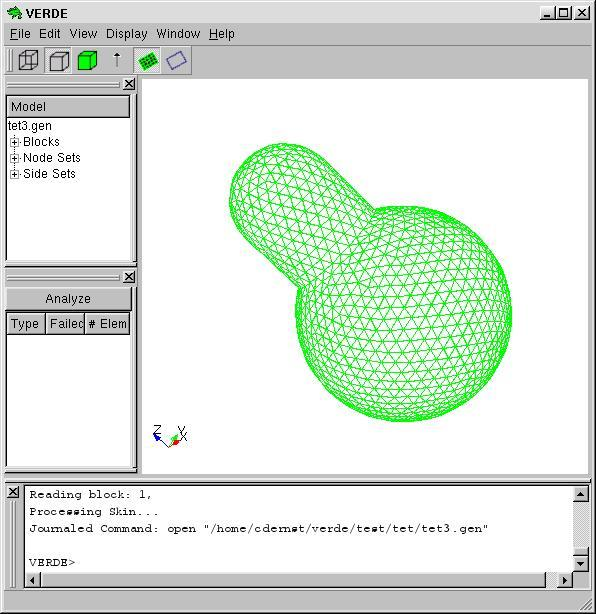
\includegraphics[height=3.8in]{images/model_screen.eps}}
              {\htmlimage[hspace=3]{images/model_screen.jpg}}
    \caption{Model skin displayed in hidden line mode.}
    \label{fig:model_screen}
  \end{center}
\end{figure}     



\subsubsection{Play Journal File}
\label{play_journal}

The Play Journal File option brings up a file open dialog that allows 
the user to select a journal file and replay a set of predefined Verde 
commands that are stored in that file.  

Appendix C gives a description of the commands used in a journal file.

\subsubsection{Record Journal File}
\label{record_journal}

The Record Journal File option brings up a file save dialog that allows 
the user to specify a file to save the commands used during a Verde 
session.  As soon as this file is opened, all journal commands are 
written into this file.  Note that most graphics manipulation commands 
are not supported in journal files in Verde version 2.6.


\subsubsection{End Record Journal File}
\label{stop_journal}

This option stops the journaling process.  No additional commands are 
written to the specified journal file.

\subsubsection{Save Mesh}
\label{save_mesh}

The save mesh command saves the currently active blocks, sidesets, and
nodesets to an Exodus II file.

\subsubsection{Save Image As}
\label{save_image}

This menu item allows the user to save the currently displayed view as 
a PNG or JPEG image file.  An extension (either .png or .jpg) 
will be appended to the file name if 
the extension doesn't already exist.  These image formats can be imported 
into many display and manipulation programs including the Microsoft 
Office Suite$^{TM}$.


\subsubsection{Print}
\label{print}

The print option brings up a print dialog and 
allows the user to print the currently 
displayed image or save the print image to a file.  This method 
currently prints a raster display of the image, so some degradation of 
image quality may occur due to the printer resolution.  

If the image is displayed on the default black background, a message 
box is displayed that allows the selection of a white background.  If 
the user clicks yes in this message box the display region will 
momentarily flash with a white background.  The image will then be 
printed in the current line color and a white background.

Note:  Verde 2.6 does not currently provide a method of printing the 
results of metrics or topology calculation.   To print this data, the 
user must select and cut the desired information from the Command Line 
window and paste it into a separate application (the editor or word 
processor of choice) for printing.

\subsubsection{Exit}
\label{exit}

Exits Verde. If Save Settings on Exit toggle (see section \ref{preferences}) 
is on, Verde saves settings information out to file, otherwise no state 
or data is saved.

\subsection{Edit Menu}
\label{edit_menu}

The Edit menu allows users to control and save parameters that are 
used by Verde during mesh verification sessions.


\subsubsection{Metric Ranges}
\label{metric_ranges}

Pass/fail criteria for the element metrics are based on the ranges that 
are defined for each metric.  The minimum and maximum acceptable range 
for each element and metric can be defined by invoking the Metric 
Ranges dialog.  This dialog box is shown in figure \ref{fig:metric_ranges}.  
The Metric 
Ranges dialog contains tabs for each element type that is supported by 
Verde.  Each tab contains fields for the minimum and maximum acceptable 
range for each metric.  Clicking either the OK or Apply buttons activates 
the changed values.  The Restore button restores the values to the 
default state.  Verde 2.6 does not yet support interactively writing or 
reading values from the .verde file.  However, this file is read at 
start up and the values are displayed in the Metrics Ranges dialog and 
used for metrics calculations.

\htmlrule
\begin{figure}[tbh]
  \begin{center}
    \texorhtml{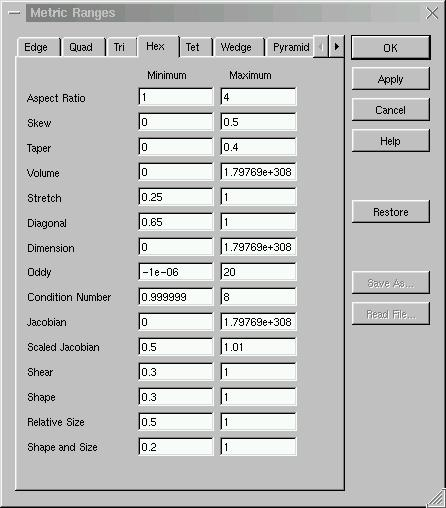
\includegraphics[height=4.0in]{images/metric_ranges.eps}}
              {\htmlimage[width=400 hspace=3]{images/metric_ranges.jpg}}
    \caption{Metric Ranges dialog box.}
    \label{fig:metric_ranges}
  \end{center}
\end{figure}     


\xname{verde_prefs}
\subsubsection{Preferences}
\label{preferences}

The Preferences dialog box is shown in figure \ref{fig:preferences}.  
This dialog box can 
be used to specify the types of calculations that Verde will perform, 
the data that should 
be echoed to the Command Window, and the user's choice of metrics 
ranges files.  The user can also set the size of points Verde draws, when
nodesets and nodes are drawn.
In Verde 2.6, the warning level was replaced with the option to specify
how intensive the check for quadrilaterals sharing three nodes is.

\htmlrule
\begin{figure}[tbh]
  \begin{center}
    \texorhtml{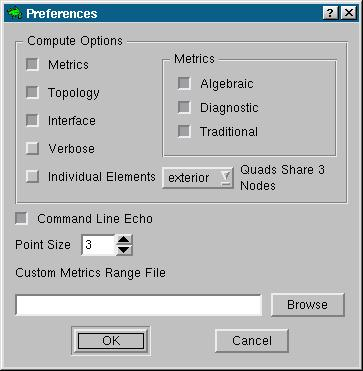
\includegraphics[width=3.0in]{images/preferences.eps}}
              {\htmlimage[width=300 hspace=3]{images/preferences.jpg}}
    \caption{Preferences dialog box.}
    \label{fig:preferences}
  \end{center}
\end{figure}     

\subsubsection{Mouse Buttons}
\label{mouse_buttons}

The Mouse Button dialog box, as show in figure \ref{fig:mouse_buttons} 
allows the user to manipulate the mapping of the mouse buttons to model 
translation, rotation, and zooming.  In addition the user can change 
the Zoom Direction (if moving the mouse up (or foward) should cause zooming 
to be positive or negative).


\htmlrule
\begin{figure}[tbh]
  \begin{center}
    \texorhtml{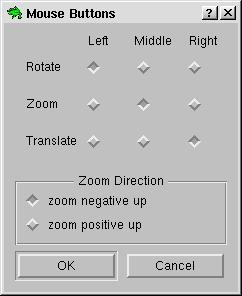
\includegraphics[width=2.5in]{images/mouse_buttons.eps}}
              {\htmlimage[width=300 hspace=3]{images/mouse_buttons.jpg}}
    \caption{Mouse Button dialog box.}
    \label{fig:mouse_buttons}
  \end{center}
\end{figure}     


\subsubsection{Save Setting on Exit}
\label{save_settings}

When exiting, if the Save Settings on Exit option it toggled on, the following 
settings are written to a file.  These setting are read in again the next time 
Verde is invoked.

%\begin{tabular}{p{4in}}
%$\bullet$ location and size of Verde main window \\
%$\bullet$ location, size, and docking status of the Model Window, 
%        Results Window, and Command Line Window \\
%$\bullet$ mapping of mouse buttons and zoom direction \\
%$\bullet$ point size \\
%$\bullet$ display toggle of normals, edges, and skin \\
%$\bullet$ Save Setting on Exit toggle \\
%$\bullet$ Perspective View toggle \\
%$\bullet$ Autofit toggle \\
%$\bullet$ Graphics mode (Hiddenline, SmoothShade or Wireframe) \\
%\end{tabular}
\begin{itemize}
\item location and size of Verde main window 
\item {location, size, and docking status of the Model Window, 
       Results Window, and Command Line Window}
\item mapping of mouse buttons and zoom direction 
\item point size 
\item display toggle of normals, edges, and skin 
\item Save Setting on Exit toggle 
\item Perspective View toggle 
\item Autofit toggle  
\item Quick Transform toggle
\item Graphics mode (Hiddenline, SmoothShade or Wireframe) 
\end{itemize}


\subsection{View Menu}
\label{view_menu}

\subsubsection{Perspective View}
\label{perspective_menu}

Perspective view can be toggle on or off.  When off, viewing is orthographic (lines 
perpendicular to the screen do not appear to converge). 

\subsubsection{AutoFit}
\label{autofit_menu}
Verde's AutoFit option centers and zooms drawn entities after issuing a graphics command 
that causes the screen to redraw, as with:

\begin{itemize}
\item activating or deactivating element blocks, 
\item {issuing a draw command (ie the command 'draw (hex$|$tet$|$wedge$|$
       pyramid$|$knife$|$quad$|$tri$|$edge$|$node) $<$range$>$') from the 
       command window.}
\end{itemize}

\subsubsection{Quick Transform}
\label{quick_transform}
This toggle controls whether mouse activated transformations (rotate, pan, or zoom)
display the entire model or just the model edges.  Transformations occur much more
smoothly and quickly if only the model edges are displayed during the transformation 
process.  The surface model can be displayed during transformations by toggling this
option off.

\subsubsection{Reset}
\label{reset}

This function returns the graphics model to its default rotation, 
scale, and translation, such that the model center is located at the 
center of the display region.

\subsection{Display Menu}
\label{display_menu}

The Display Menu controls how the graphics are displayed in the display 
region.  The display region is drawn using the portable OpenGL$^{TM}$
graphics API.  


\subsubsection{Wireframe/Hidden/Smooth Shade}
\label{mode}


These toggle actions control how the model is displayed.  The graphics 
modes can be controlled from both the Display menu and the Verde 
toolbar.  

\subsubsection{Normals}
\label{normals}
This menu item toggles the display of normal vectors on the model.  
Figure \ref{fig:normals} shows an example of this type of display.

\subsubsection{Skin}
\label{skin}
This menu item toggles the skin on or off.  Turning off the skin can 
be useful for visualizing failed elements or interfaces internal to
the model.

\subsubsection{Model Edges}
\label{edges}
This menu item toggles the model edges on or off.  Turning off the skin and
turning on the model edges 
is useful for visualizing failed elements or interfaces internal to
the model.

Verde displays both inferred edges and free edges, edges which belong
to only one polygon.
The inferred model edges are determined by calculating feature 
angles between adjacent
polygons.  This can cause problems if the object is primarily smooth.
For example the object displayed in figure \ref{fig:model_screen} only
has one edge as shown in figure \ref{fig:edge_only}

\htmlrule
\begin{figure}[tbh]
  \begin{center}
    \texorhtml{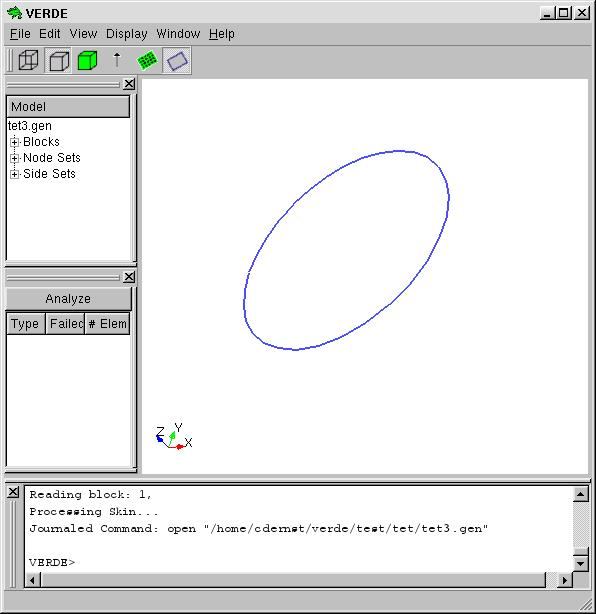
\includegraphics[height=3.8in]{images/edge_only.eps}}
              {\htmlimage[hspace=3]{images/edge_only.jpg}}
    \caption{Edge calculated for a relatively smooth object.}
    \label{fig:edge_only}
  \end{center}
\end{figure}     
\htmlrule

\subsubsection{Labels}
\label{labels}
Verde can display labels (ids) of the following entities:

\begin{itemize}
\item nodesets
\item sidesets 
\item blocks
\item failed elements
\item nodes
\item elements
\end{itemize}

Node and element ids are based on the implicit numbering present
in the Exodux II file.  The ids are not based on any mapping defined
in a prior application.  Element ids are unique for all element topologies
so that no element id duplicated.  For example, a quad and a hex cannot
share the same id number.

\subsubsection{Background Color}
\label{colors}

The display menu also provides methods of setting the  
background color of the display area via a color dialog box as shown in figure
\ref{fig:color_dlg}.

\htmlrule
\begin{figure}[tbh]
  \begin{center}
    \texorhtml{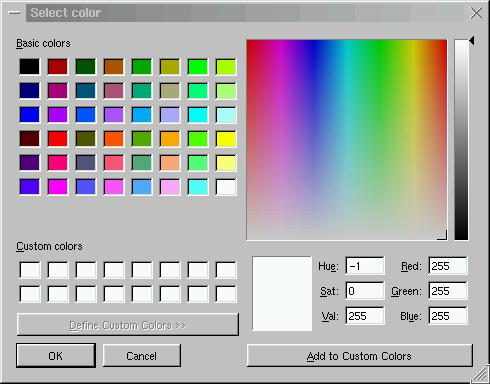
\includegraphics[width=4.0in]{images/color_dlg.eps}}
              {\htmlimage[width=400 hspace=3]{images/color_dlg.jpg}}
    \caption{Select Color dialog for foreground and background colors.}
    \label{fig:color_dlg}
  \end{center}
\end{figure}     
\htmlrule

The background can be set to any color by choosing 
either one of the predefined colors in the color table or by creating a 
custom color.  Note that in version 2.6 of Verde the custom colors are 
not maintained between sessions.


\subsubsection{Model Manipulation}
\label{manipulation}

In addition to the display options that are available from the Display 
menu, the graphics model may also be transformed using the mouse.  


\begin{center}
\begin{tabular}{ll}
Left mouse:   & Rotation about the model X and Y axes.  \\
Right mouse:  & Translation in the screen X and Y axes. \\
Middle mouse: & Zoom in the screen Z axis.              \\
\end{tabular}
\end{center}


The mapping of mouse button to transformation can be defined 
by the user as described in section \ref{preferences}.


\subsection{Windows}
\label{windows}

This menu item controls the display of the three dockable windows.  Toggling
an item off removes it from the display.

\subsection{Help}
\label{help}

Displays this document.

The help system should be configured properly by the install
process.  However, if an error should occur check the following
items.

\begin{enumerate}
  \item The environmental variable VERDE\_DIR should point to the
	directory where the verde executable is located.  The 
	documentation (verde*.html) is located in a
	sub-directory  of VERDE\_DIR named {\it doc} (\$VERDE\_DIR/doc).
  \item The helper application {\it verde\_help} should exist in the
	VERDE\_DIR directory.
\end{enumerate}

If either of these items is incorrect, you can correct the problem
manually or attempt to reinstall verde.

\xname{verde_batch}
\chapter{Controlling Verde in Batch Mode} 
\label{sec:batch}


Verde can be run as a batch-mode program when invoked from the command 
prompt with the ``--batch'' option.

The basic syntax of the Verde batch command is:
\footnote %What do we do with this?
{
Under MS Windows$^{TM}$ operating systems users should run verde, as
documented, and {\bf not} verde.exe.  The batch version is 
run from verde.com.  This file provides console output
capabilities (such as redirection and pipe) similar to the UN*X
console mode.  The verde.com file resides in the
same directory as the verde executable.
}


\begin{center}

\% verde --batch [options] input\_file.gen
\end{center}

where input\_file is the file to be verified (in Exodus II format) and 
the options are optional control flags.  Options are preceded by the 
``-`` character (``minus'' or ``dash'') and can be specified in any 
order. Current valid options for version 2.6 are:

\begin{center}
\begin{tabular}{lp{4in}}
-help            & Print this summary                                     \\
-batch           & Runs verde in batch mode                               \\
-blocks $<$\$val$>$  & Specifies block(s) to be processed (e.g. 1,5-7,9)  \\
-individual      & prints metrics for each block individually             \\
-list\_defaults  & Lists defaults settable in .verde defaults file        \\
-defaults $<$\$val$>$ & Specifies path and file of defaults file (e.g ../defaults1) \\
-nodefaults      & do not process .verde default file                     \\
-nointerface     & Suppresses mesh interface verification calculations    \\
-nometrics       & Suppresses element metric calculations                 \\
-output $<$\$val$>$ & Generates an Exodus II output file specified by $val$   \\
-notopology &Suppresses mesh topology verification calculations           \\
-print\_failed\_elements & Prints individual failed elements and values   \\
-version                 & Prints the verde version number                \\
-quads\_share\_3\_nodes $<$\$val$>$ & Check entire mesh, exterior quads, 
or nothing for quads sharing 3 nodes (all, exterior, none)                   \\
\end{tabular}
\end{center}

Used without any options, e.g.,

\begin{center}
\% verde --batch test\_file.gen
\end{center}

Verde will perform all available verification procedures to the file 
test\_file.gen.  The most common options are specified to suppress one 
or more verification procedures on the file.  For large files, the 
savings in execution time resulting from suppressing verification 
procedures can become important.

\chapter{Program Output}
\label{sec:output}

When Verde is used to verify a mesh, by default it sends output to the 
command line and optionally (using -output) to an auxiliary graphics 
output file.  Option flags control the exact output at the command 
line, and can also be used to disable the graphics file output.


\section{GUI Output}
\label{gui_output}
The graphical user interface provides a method of
visualizing the results from a Verde analysis.  After clicking
on the Analyze button, failure cases are listed in the Results
window.  If nothing is listed, the model passed all tests for
the currently defined set of metric ranges.
The results from the graphical user interface are 
primarily based on the visual display of the results data.
The results to be displayed are selected by clicking on one
of the items in the Results window. If there are no items
displayed the model passes all requested tests.

By default, element metric, topological, and interface analyses
are performed on the model.  Specific analyses may be excluded 
by deselecting them in the \xlink{Edit/Preferences}{verde_prefs.html} 
dialog box.

The following sections outline the types of results that
are available for each analysis type.

\subsection{Individual Element Metrics} 
The results for individual element metrics can be displayed
by clicking on the appropriate entry in the Results window.
An example of the resulting display is shown in figure 
\ref{fig:element_metrics}.  This display was created by turning
model shell off and rendering the failed elements in hidden
line mode.  This provides a useful method of viewing bad elements
internal to the model.

\htmlrule
\begin{figure}[tbhp]
  \begin{center}
    \texorhtml{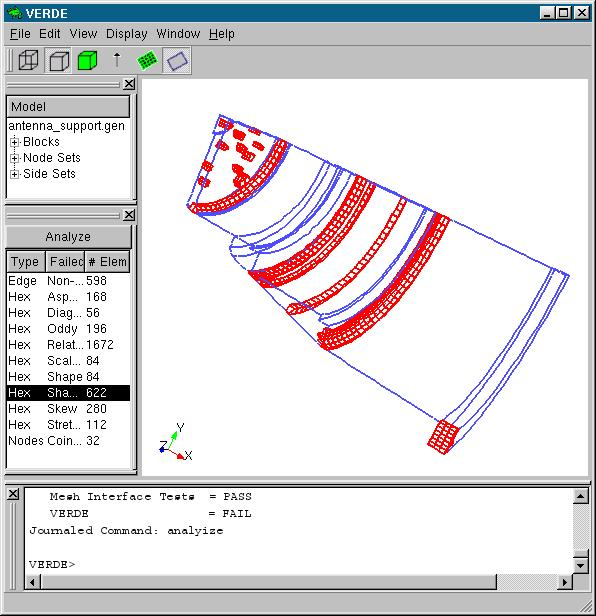
\includegraphics[height=3.7in]{images/element_metrics.eps}}
              {\htmlimage[hspace=3]{images/element_metrics.jpg}}
    \caption{Sample results display of failed elements.}
    \label{fig:element_metrics}
  \end{center}
\end{figure}     
\htmlrule

\subsection{Topology Checks} 

A topological analysis is performed that determines if the
model is manifold, composed of complete solids or shells,
or non-manifold.  Non-manifold objects may include a mixture
of bar, shell and/or solid elements, or they may be objects that are
not correctly closed.  Non-manifold edges may indicate the presence 
of  hinges in the model.

The command window prints a prediction of the probable topology of the model.
For example, the topology information for figure \ref{fig:normals} 
is calculated as:

\begin{example}
----------------------------
Mesh Topology Information
----------------------------
   Probable Topology:  Open Surface with 11 hole(s)
   Possible Topologies: N Open surfaces with N+10 hole(s)
\end{example}

This calculation is based on the Euler-Descartes formula $E= v - e + f$,
where $v$ is the number of vertices, $e$ is the number of edges, and
$f$ is the number of faces\cite{CRC}.

Verde 2.6 can display non-manifold edges as shown in figure 
\ref{fig:nonmanifold}.  
A non-manifold edge occurs when more than two entities share a 
boundary edge.
The figure shows two blocks that are only
connected along one edge.  This is not a valid solid object.  If the 
model is not properly constrained, it could result in a hinge that
may cause some analysis codes to fail.

\htmlrule
\begin{figure}[tbhp]
  \begin{center}
    \texorhtml{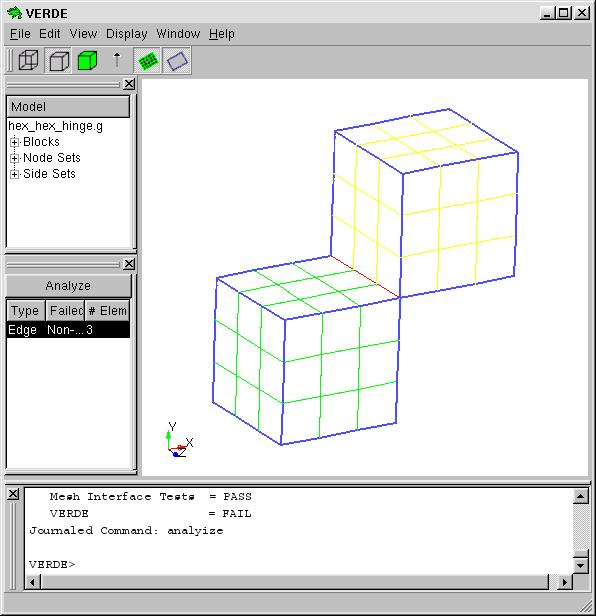
\includegraphics[height=3.7in]{images/nonmanifold.eps}}
              {\htmlimage[hspace=3]{images/nonmanifold.jpg}}
    \caption{Display of non-manifold edges.}
    \label{fig:nonmanifold}
  \end{center}
\end{figure}     
\htmlrule

Figure \ref{fig:quads_on_hexes} demonstrates another case that
reports non-manifold edges in Verde 2.6.  In this case there
are shell elements superimposed on a set of hexahedral elements.  
Once again, this may be correct, but it allows the user to verify 
that the desired elements are in the correct location.  Bar elements
which share an edge with other elements will also be flagged as
non-manifold entities.

\htmlrule
\begin{figure}[tbhp]
  \begin{center}
    \texorhtml{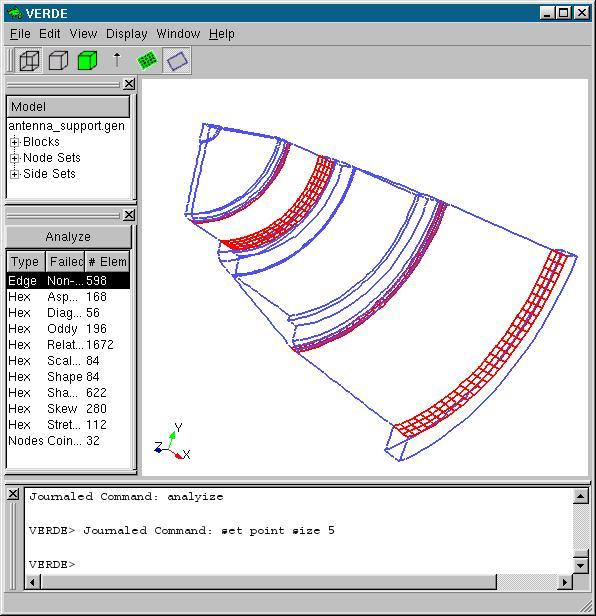
\includegraphics[height=3.7in]{images/quads_on_hexes.eps}}
              {\htmlimage[hspace=3]{images/quads_on_hexes.jpg}}
    \caption{Display of shell elements superimposed on hex elements.}
    \label{fig:quads_on_hexes}
  \end{center}
\end{figure}     
\htmlrule

The topology of a model can also be checked by 
displaying the element normals.  Figure \ref{fig:normals} shows a shell
model with the normals turned on.  Note that in the upper left hand
corner the normals of the flange have the opposite sense of the normals
on the rest of the model.  Inverted normals can cause some analysis 
programs to calculate negative areas for some of the elements and may
result in an aborted analysis.
\htmlrule
\begin{figure}[tbhp]
  \begin{center}
    \texorhtml{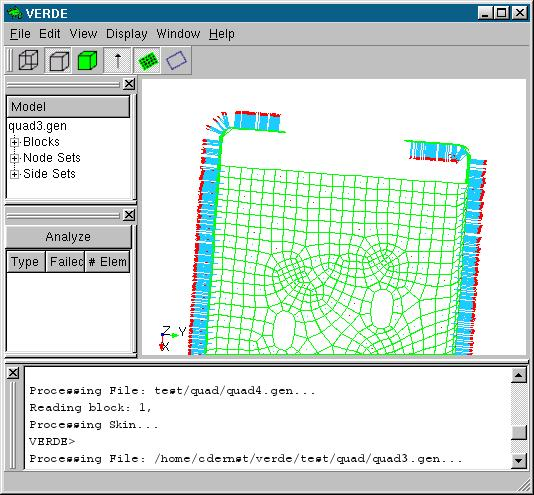
\includegraphics[height=3.7in]{images/normals.eps}}
              {\htmlimage[hspace=3]{images/normals.jpg}}
    \caption{Display of element normals on a shell model.}
    \label{fig:normals}
  \end{center}
\end{figure}     
\htmlrule

\subsection{Interface Checks} 

Verde 2.6 also provides tools to verify the interfaces between
sections of a model.  Figure \ref{fig:coincident_nodes} shows 
red squares at locations where two nodes are coincident.  This may
not necessarily be an error in the model if the nodes are in sliding
contact or are constrained by some type of multi-point constraint.

\htmlrule
\begin{figure}[tbhp]
  \begin{center}
    \texorhtml{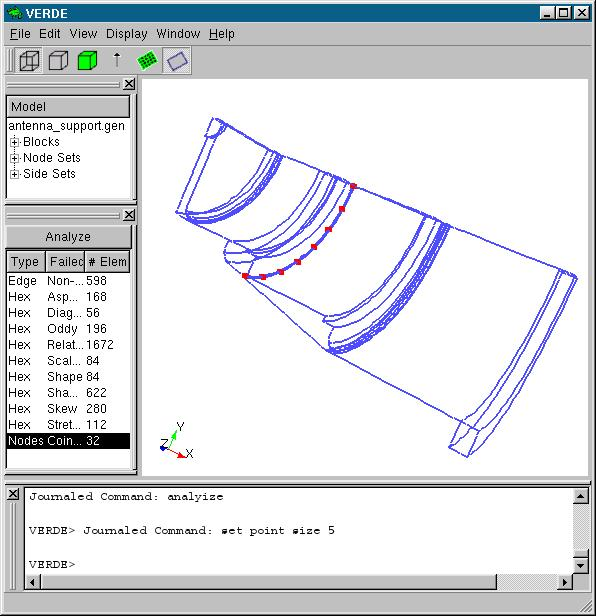
\includegraphics[height=3.7in]{images/coincident_nodes.eps}}
              {\htmlimage[hspace=3]{images/coincident_nodes.jpg}}
    \caption{Display of coincident nodes in model.}
    \label{fig:coincident_nodes}
  \end{center}
\end{figure}     
\htmlrule

%If coincident nodes occur in the model, there may also be coincident edges.
%Coincident edges occur if both endpoints are coincident with another edge.
%This may indicate that the model is non-conformal.

% Also checks for non-conformal tris.

Verde also detects coincident quadrilaterals and triangles.  This may 
indicate that the model is not correctly joined.

\subsection{Quadrilaterals Sharing 3 Nodes}

Verde 2.6 can check for interface problems between adjoining 
hexahedral elements.  It can also check for quadrilaterals that make up the surface of the mesh which share 3 nodes.  Figure \ref{fig:quad_3_nodes} shows the faces of
adjoining hexahedral highlighted which share only 3 nodes.

\htmlrule
\begin{figure}[tbhp]
  \begin{center}
    \texorhtml{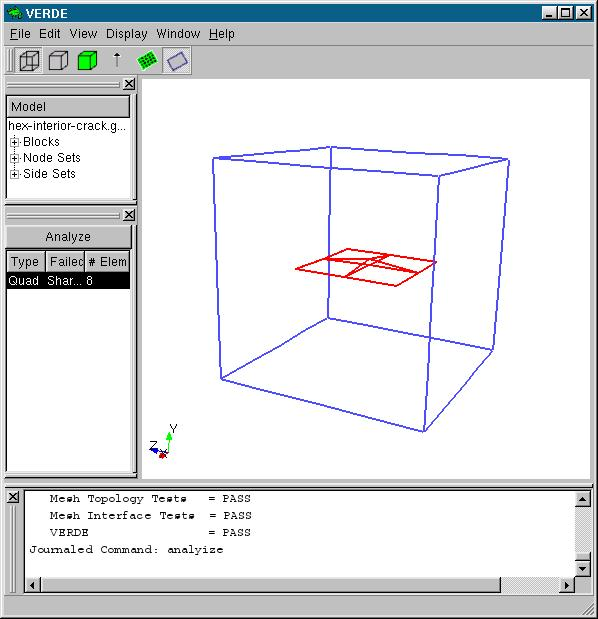
\includegraphics[height=3.7in]{images/quad_3_nodes.eps}}
              {\htmlimage[hspace=3]{images/quad_3_nodes.jpg}}
    \caption{Display of quadrilaterals sharing three nodes in model.}
    \label{fig:quad_3_nodes}
  \end{center}
\end{figure}     
\htmlrule


\section{Command Line Output}
\label{command_line}

Command line output is divided into seven sections:


\begin{enumerate}


\item
{
Banner:  This prints the version of Verde being run, the revision date 
of Verde, and the execution date of the run.
}
\item
{
Element Metrics: In this section, metric information is output for each 
element type in the input file. If the -individual option is used, 
metric information is output for each individual element block.
}
\item
{
Metric Summary:  This section lists information about the number of 
elements of each type that fail the various metric tests.  If the 
-verbose option flag is specified, each element is listed, along with 
the failed metric value for the element.
}
\item
{
Mesh Topology Information:  This section lists any possible topology 
problems found in the mesh, and states whether the mesh appears to be 
conformal or not.  The probable topology of the mesh model is also 
listed based on the Euler number calculated for this body.
}
\item
{
Mesh Interface Information:  This section gives summary information 
about the exterior skin of the model and the inferred model edges 
found.  If any potential problems with the exterior are discovered 
(such as incomplete or incorrect mesh joining, non-conformal 
interfaces, etc) these are listed as warnings.
}
\item
{
Output Information:  Verde can generate an Exodus II file during an 
analysis of all failed elements.  This file is organized into blocks.
Block 1 contains the model skin. Block 2 contains the edges of the 
model.  Blocks 3 to n contain failed elements for each of the 
metrics that have failed elements. The file is written only if 
the -output option is used when invoking verde.
}
\item
{
Execution Summary:  This section lists summary information about the 
size and execution speed of the run, and gives a summary of each 
verification procedure, listing the result as PASS, FAIL, or WARN, as 
well as an overall PASS/FAIL for the Verde run.  If any FAIL or WARN 
occurs in any verification procedure, the overall Verde run is flagged 
as FAIL.  NOTE: A failure condition in Verde does not always mean the 
mesh is incorrect.  For example, a mesh with contact surfaces would 
generate a WARN in the Mesh Interface Information section, but would be 
a valid mesh for the problem.
}
\end{enumerate}


Listed below is the output for a sample run of Verde:


\begin{example}
\small{

\% verde -batch -output output_file.gen antenna_support.gen


		         *** VERDE Version 2.6 ***

		        Revised 05-16-02 03:30:57 PM

		VERDE: VERIFICATION OF DISCRETE ELEMENTS

		A MESH VERIFICATION TOOL FOR EXODUS MESHES

		      Executing on 05/17/02 at 12:48:14 PM

		This version of Verde is only for use inside Sandia

Executing: /home/kgmerk/verde/verde_exe -batch -output output_file.gen antenna_support.gen 

Processing File: antenna_support.gen...
Reading block: 1, 2, 3, 4, 5, 6, 7, 8, 9, 10,
Processing Skin...

---------------
Element Metrics
---------------
Processing block 1, 261 elements of type HEX:

Processing block 2, 84 elements of type SHELL:

Processing block 3, 616 elements of type SHELL:

Processing block 4, 56 elements of type SHELL:

Processing block 5, 1820 elements of type HEX:

Processing block 6, 588 elements of type HEX:

Processing block 7, 84 elements of type SHELL:

Processing block 8, 189 elements of type SHELL:

Processing block 9, 21 elements of type SHELL:

Processing block 10, 1039 elements of type HEX:


Summary Hex Metrics, total = 3708 Hexes:

   Function Name     Average    Std Dev    Minimum   (id)  Maximum  (id)
 -----------------  ---------  ---------  --------------  -------------

ALGEBRAIC METRICS
             Shear  0.9238993   0.10812   0.5168335 (391)  0.9997690 (3113)
             Shape  0.7674397   0.18242   0.2528860 (299)  0.9794520 (2935)
     Relative Size  0.6983444   0.17324   0.1998347 (4)  0.9737509 (3059)
    Shape and Size  0.5507035   0.19747   0.0749352 (333)  0.8845074 (3059)

DIAGNOSTIC METRICS
    Element Volume  0.0027304   0.00168   0.0004244 (3654)  0.0093638 (57)

TRADITIONAL METRICS
      Aspect Ratio  2.0273290   0.87532   1.0112389 (2979)  5.3614430 (398)
              Skew  0.1713917   0.18155   0.0000930 (3106)  0.7829728 (421)
             Taper  0.0090899   0.00953   0.0000000 (1)  0.0346601 (2857)
           Stretch  0.6235547   0.16580   0.1858189 (300)  0.8732918 (3665)
    Diagonal Ratio  0.9264883   0.07396   0.6338562 (601)  0.9999243 (3106)
         Dimension  0.0707981   0.01839   0.0325387 (327)  0.1062584 (57)
              Oddy  4.4684236   9.23531   0.1271596 (2978)  52.721605 (401)
     Condition No.  1.4180944   0.51873   1.0209791 (2935)  3.9543516 (299)
          Jacobian  0.0022765   0.00157   0.0003001 (3654)  0.0086663 (57)
   Scaled Jacobian  0.9003169   0.13206   0.4421353 (391)  0.9996536 (3113)

Summary Quad Metrics, total = 1050 Quads:

   Function Name     Average    Std Dev    Minimum   (id)  Maximum  (id)
 -----------------  ---------  ---------  --------------  -------------

ALGEBRAIC METRICS
             Shear  1.0000000   0.00000   1.0000000 (88)  1.0000000 (88)
             Shape  0.9177645   0.04264   0.7638335 (738)  0.9627218 (4004)
     Relative Size  1.0000000   0.00000   1.0000000 (88)  1.0000000 (88)
    Shape and Size  0.9177645   0.04264   0.7638335 (738)  0.9627218 (4004)

DIAGNOSTIC METRICS
      Element Area  0.0299522   0.00229   0.0222158 (738)  0.0313723 (6820)

TRADITIONAL METRICS
      Aspect Ratio  1.5180575   0.17941   1.3196892 (4004)  2.1541519 (738)
              Skew  0.0000000   0.00000   0.0000000 (88)  0.0000000 (88)
             Taper  0.0000000   0.00000   0.0000000 (88)  0.0000000 (88)
           Warpage  1.0000000   0.00000   1.0000000 (88)  1.0000000 (88)
           Stretch  0.7817586   0.05724   0.5954718 (738)  0.8541115 (4004)
     Maximum Angle  90.000000   0.00001   90.000000 (88)  90.000000 (88)
     Minimum Angle  90.000000   0.00001   90.000000 (88)  90.000000 (88)
              Oddy  0.3926366   0.26880   0.1578855 (4004)  1.4279352 (738)
     Condition No.  1.0922582   0.05739   1.0387217 (4004)  1.3091859 (738)
          Jacobian  0.0299522   0.00229   0.0222158 (738)  0.0313723 (6820)
   Scaled Jacobian  1.0000000   0.00000   1.0000000 (88)  1.0000000 (88)

---------------
Metrics Summary
---------------
   Number of Failed Hex Metrics: 1755
      Failed Shape: 28  	(valid range:      0.300 to      1.000)
      Failed Relative Size: 545  	(valid range:      0.500 to      1.000)
      Failed Shape and Size: 286  	(valid range:      0.200 to      1.000)
      Failed Aspect Ratio: 168  	(valid range:      1.000 to      4.000)
      Failed Skew: 280  	(valid range:      0.000 to      0.500)
      Failed Stretch: 112  	(valid range:      0.250 to      1.000)
      Failed Diagonal Ratio: 56  	(valid range:      0.650 to      1.000)
      Failed Oddy: 196  	(valid range:      0.000 to     20.000)
      Failed Scaled Jacobian: 84  	(valid range:      0.500 to      1.010)
   Number of Failed Quad Metrics: 0

----------------------------
Quads Sharing 3 Nodes
----------------------------
   Number Quads sharing three nodes:  0

----------------------------
Mesh Topology Information
----------------------------
   Topology: Non-Manifold
   Number Non-Manifold Edges:  598

-------------------------
Mesh Interface Information
-------------------------
   Number Surface Quads:     4448
   Number Surface Tris:      0
   Number Coincident Nodes:  32
   Number Coincident Quads:   0
   Number Coincident Tris:   0
   Number Model Edges:       1150



------------------
Output Information
------------------
   Writing Output to exodus file output_file.gen:
   Writing 4830 exterior nodes...
   Writing 4448 exterior quads to block 1...
   Writing 1150 model edges to block 2...
   Writing 28 failed hexes (Shape) to block 3...
   Writing 545 failed hexes (Relative Size) to block 4...
   Writing 286 failed hexes (Shape and Size) to block 5...
   Writing 168 failed hexes (Aspect Ratio) to block 6...
   Writing 280 failed hexes (Skew) to block 7...
   Writing 112 failed hexes (Stretch) to block 8...
   Writing 56 failed hexes (Diagonal Ratio) to block 9...
   Writing 196 failed hexes (Oddy) to block 10...
   Writing 84 failed hexes (Scaled Jacobian) to block 11...

-----------------
Execution Summary
-----------------
   User time             = 2.25
   Elements Processed    = 4758
   Elements Per Second   = 2114
   Total Volume          = 10.12
   Total Area            = 31.45

   Metrics Tests         = FAIL  (see Metrics Summary above)
   Mesh Topology Tests   = FAIL (see Mesh Topology Information above)
   Mesh Interface Tests  = PASS
   VERDE                 = FAIL

}
\end{example}

\T\begin{appendix}
\chapter{The .verde Preferences File}
\label{sec:verde_prefs}

For Verde version 2.6, the .verde preferences file format has been changed
to a journal file format.  \footnote { A utility is provided to convert old
 preferences files into the new format.  Usage is: defaults\_converter2\_5 
-o OutputFile InputFile }

The .verde preferences file can be used to customize the behavior of 
Verde to a large extent.  Verde looks for a valid verification file 
first in the current working directory (./.verde) and then in the home 
directory (\$(HOME)/.verde).  If a valid file is found, it is processed 
first, before any flags on the command line.  Therefore, if an option 
is listed in both the .verde file and on the command line, the command 
line flag will take precedence.  The .verde file can set the same flags 
as are available on the command line.  It is also possible to control 
the valid range of any Verde metric using the file.  Thus, if there are 
certain element metric limits for a given application, these can be 
stored in the .verde file and used in place of the default limits.

Below is an example journal file which sets topology calculations on, 
interface calculations off, metric calculations on, sets the hexahedral 
aspect range, and sets the tetrahedral Jacobian range.

\begin{example}
# Command Line Flags:
set topology\_calculations on
set interface\_calculations off
set metric\_calculations on
# Hex Metrics failure criteria:
set hex aspect minimum .5
set hex aspect maximum 1
# Tet Metrics failure criteria:
set tet jacobian minimum .8
set tet jacobian maximum 1

\end{example}


\T\newpage
\chapter{Descriptions of Verde Metrics}
\label{sec:appendix_B}


The following tables provide a description of the metrics that
are applicable to each element type.  Table \ref{tab:hex}
lists the metrics that are applicable to hexahedral meshes.  

\begin{table}[h]
\begin{center}
\begin{tabular}{|l|c|c|c|c|}
\hline
Function Name  &  Dimension & Full Range &Acceptable Range &  Reference \\
\hline
Aspect Ratio   &    $L^0$ &    1 to inf  &    1 to 4       & \cite{taylor} \\
Skew           &    $L^0$ &    0 to 1    &    0 to 0.5     & \cite{taylor} \\
Taper          &    $L^0$ &    0 to +inf &    0 to 0.4     & \cite{taylor} \\
Element Volume &    $L^3$ & -inf to +inf &     None        & \cite{taylor} \\
Stretch        &    $L^0$ &    0 to 1    &  0.25 to 1      & \cite{fimesh} \\
Diagonal Ratio &    $L^0$ &    0 to 1    &  0.65 to 1      &            \\
Dimension      &    $L^1$ &    0 to inf  &     None        & \cite{taylor} \\
Oddy           &    $L^0$ &    0 to inf  &    0 to 20      & \cite{oddy}\cite{knupp2000} \\
Condition No.  &    $L^0$ &    1 to inf  &    1 to 8       & \cite{knupp2000} \\
Jacobian       &    $L^3$ & -inf to inf  &     None        & \cite{knupp2000} \\
Scaled Jacobian&    $L^0$ &   -1 to +1   &  0.5 to 1       & \cite{knupp2000} \\
Shear          &    $L^0$ &    0 to 1    &  0.3 to 1       & \cite{knupp2002} \\
Shape          &    $L^0$ &    0 to 1    &  0.3 to 1       & \cite{knupp2002} \\
Relative Size  &    $L^0$ &    0 to 1    &  0.5 to 1       & \cite{knupp2002} \\
Shape \& Size  &    $L^0$ &    0 to 1    &  0.2 to 1       & \cite{knupp2002} \\
\hline
\end{tabular}
\end{center}
\T\caption{Description of Hexahedral Quality Measures}
\htmlcaption{Description of Hexahedral Quality Measures}
\label{tab:hex}
\end{table}

The metrics for hexahedral elements as listed in table 
\ref{tab:hex} are defined as follows:
\T\bigskip
\htmlrule

\begin{tabular}{lp{4in}}
Aspect Ratio:& 
  Maximum edge length ratios at hex center. \\
Skew:      & 
  Maximum $\|\cos A\|$ where A is the angle between edges at hex center. \\
Taper:       & 
  Maximum ratio of lengths derived from opposite edges. \\
Element Volume:  & 
  Jacobian at hex center. \\
Stretch:         &  
  $\sqrt{3}$ * minimum edge length / maximum diagonal length. \\
Diagonal Ratio:  & 
  Minimum diagonal length / maximum diagonal length. \\
Dimension:       & 
  Pronto-specific characteristic length for stable time step calculation.      Char\_length = Volume / 2 grad Volume. \\
Oddy: & 
  General distortion measure based on left Cauchy-Green Tensor. \\
Condition No. & 
  Maximum condition number of the Jacobian matrix at 8 corners. \\
Jacobian: & 
  Minimum pointwise volume of local map at 8 corners \& center of hex. \\
Scaled Jacobian:& 
  Minimum Jacobian divided by the lengths of the 3 edge vectors. \\
Shear:           & 
  3/Condition number of Jacobian Skew matrix \\
Shape:           & 
  3/Condition number of weighted Jacobian matrix \\
Relative Size:   & 
  Min( J, 1/J ), where J is determinant of weighted Jacobian matrix \\
Shape and Size:  & 
  Product of Shape and Relative Size \\
\end{tabular}
\T\newpage
\htmlrule

Table \ref{tab:quad}
lists the metrics that are applicable to quadrilateral meshes.  

\begin{table}[h]
\begin{center}
\begin{tabular}{|l|c|c|c|c|}
\hline
Function Name   & Dimension & Full Range &Acceptable Range &  Reference \\
\hline
Aspect Ratio    &   $L^0$ &    1 to inf  &    1 to 4    & \cite{robinson} \\
Skew            &   $L^0$ &    0 to 1    &    0 to 0.5  & \cite{robinson} \\
Taper           &   $L^0$ &    0 to inf  &    0 to 0.7  & \cite{robinson} \\
Warpage         &   $L^0$ &    0 to inf  &    0 to 0.1  & \cite{robinson} \\
Element Area    &   $L^2$ & -inf to +inf &     None     & \cite{robinson} \\
Stretch         &   $L^0$ &    0 to 1    & 0.25 to 1    &                 \\
Minimum Angle   &  degrees&   0 to 90    &  45 to 90    &         \\
Maximum Angle   &  degrees&  90 to 360   &  90 to 135   &         \\
Oddy            &   $L^0$ &    0 to inf  &    0 to 16   & \cite{oddy}\cite{knupp2000} \\
Condition No.   &   $L^0$ &    1 to inf  &    1 to 4    & \cite{knupp2000} \\
Jacobian        &   $L^2$ & -inf to inf  &     None     & \cite{knupp2000} \\
Scaled Jacobian &   $L^0$ &   -1 to +1   &  0.5 to 1    & \cite{knupp2000} \\
Shear           &   $L^0$ &    0 to 1    &  0.3 to 1    & \cite{knupp2002} \\
Shape           &   $L^0$ &    0 to 1    &  0.3 to 1    & \cite{knupp2002} \\
Relative Size   &   $L^0$ &    0 to 1    &  0.5 to 1    & \cite{knupp2002} \\
Shape \& Size   &   $L^0$ &    0 to 1    &  0.2 to 1    & \cite{knupp2002} \\
\hline
\end{tabular}
\end{center}
\T\caption{Description of Quadrilateral Quality Measures}
\htmlcaption{Description of Quadrilateral Quality Measures}
\label{tab:quad}
\end{table}


The metrics for quadrilateral elements as listed in table 
\ref{tab:quad} are defined as follows:
\T\bigskip
\htmlrule

\begin{tabular}{lp{4in}}
Aspect Ratio:     & Maximum edge length ratios at quad center \\
Skew: & Maximum $\|\cos A\|$ where A is the angle between edges at quad center \\
Taper:            & Maximum ratio of lengths derived from opposite edges \\
Warpage:          & Deviation of element from planarity. \\
Element Area:     & Jacobian at quad center \\
Stretch:          & $\sqrt{2}$ * minimum edge length / maximum diagonal length\\
Minimum Angle:    & Smallest included quad angle (degrees).  \\
Maximum Angle:    & Largest included quad angle (degrees).  \\
Oddy:             & General distortion measure based on left Cauchy-Green Tensor \\
Condition No.     & Maximum condition number of the Jacobian matrix at 4 corners \\
Jacobian:         & Minimum pointwise volume of local map at 4 corners \& center of quad \\
Scaled Jacobian:  & Minimum Jacobian divided by the lengths of the 2 edge vectors \\
Shear:             & 2/Condition number of Jacobian Skew matrix \\
Shape:             & 2/Condition number of weighted Jacobian matrix \\
Relative Size:     & Min( J, 1/J ), where J is determinant of weighted Jacobian matrix \\
Shape and Size:    & Product of Shape and Relative Size \\
\end{tabular}
\T\newpage
\htmlrule


Table \ref{tab:tet}
lists the metrics that are applicable to tetrahedral meshes.  

\begin{table}[h]
\begin{center}
\begin{tabular}{|l|c|c|c|c|}
\hline
Function Name   & Dimension & Full Range &Acceptable Range &  Reference \\
\hline
Aspect Ratio Bet  & $L^0$ &     1 to inf   &   1 to 3      & \cite{parth} \\
Aspect Ratio Gam  & $L^0$ &     1 to inf   &   1 to 3      & \cite{parth} \\
Element Volume    & $L^3$ &  -inf to +inf  &    None       & \cite{parth} \\
Condition No.     & $L^0$ &     1 to inf   &   1 to 3      & \cite{knupp2000} \\
Jacobian          & $L^3$ &  -inf to inf   &    None       & \cite{knupp2000} \\
Scaled Jacobian   & $L^0$ &-1.414 to +1.414& 0.5 to +1.414 & \cite{knupp2000} \\
Shear             & $L^0$ &     0 to 1     & 0.3 to 1      & \cite{knupp2002} \\
Shape             & $L^0$ &     0 to 1     & 0.3 to 1      & \cite{knupp2002} \\
Relative Size     & $L^0$ &     0 to 1     & 0.5 to 1      & \cite{knupp2002} \\
Shape \& Size     & $L^0$ &     0 to 1     & 0.2 to 1      & \cite{knupp2002} \\
\hline
\end{tabular}
\end{center}
\T\caption{Description of Tetrahedral Quality Measures}
\htmlcaption{Description of Tetrahedral Quality Measures}
\label{tab:tet}
\end{table}

The metrics for tetrahedral elements as listed in table 
\ref{tab:tet} are defined as follows:
\T\bigskip
\htmlrule

\begin{tabular}{lp{4in}}
Aspect Ratio Beta: & CR / (3.0 * IR)  where CR = circumsphere radius, IR = inscribed sphere radius \\
Aspect Ratio Gamma:& $Srms^3 / (8.479670*V)$  where $Srms = \sqrt{Sum(Si^2)/6}$, $Si$ = edge length \\
Element Volume:    & (1/6) * Jacobian at corner node \\
Condition No.      & Condition number of the Jacobian matrix at any corner \\
Jacobian:          & Minimum pointwise volume at any corner \\
Scaled Jacobian:   & Minimum Jacobian divided by the lengths of 3 edge vectors \\
Shear:             & 3/Minimum condition number of weighted Skew matrices \\
Shape:             & 3/Condition number of weighted Jacobian matrix \\
Relative Size:     & Min( J, 1/J ), where J is determinant of weighted Jacobian matrix \\
Shape and Size:    & Product of Shape and Relative Size \\
\end{tabular}
\T\newpage
\htmlrule

Table \ref{tab:tri}
lists the metrics that are applicable to triangular meshes.  

\begin{table}[h]
\begin{center}
\begin{tabular}{|l|c|c|c|c|}
\hline
Function Name   & Dimension & Full Range &Acceptable Range &  Reference \\
\hline
Aspect Ratio Gam&  $L^0$ &     1 to inf   &     1 to 1.3   & \cite{parth} \\ 
Element Area    &  $L^2$ &     0 to inf   &      None      &        \\
Maximum Angle   & degrees&    60 to 180   &    60 to 90    &        \\
Minimum Angle   & degrees&     0 to 60    &    30 to 60    &        \\
Condition No.   &  $L^0$ &     1 to inf   &     1 to 1.3   & \cite{knupp2000} \\
Scaled Jacobian &  $L^0$ &-1.155 to +1.155&   0.5 to 1.155 & \cite{knupp2000} \\
Shear           &  $L^0$ &     0 to 1     &  0.75 to 1     & \cite{knupp2002} \\
Shape           &  $L^0$ &     0 to 1     &  0.75 to 1     & \cite{knupp2002} \\
Relative Size   &  $L^0$ &     0 to 1     &  0.75 to 1     & \cite{knupp2002} \\
Shape \& Size   &  $L^0$ &     0 to 1     &  0.75 to 1     & \cite{knupp2002} \\
\hline
\end{tabular}
\end{center}
\T\caption{Description of Triangular Quality Measures}
\htmlcaption{Description of Triangular Quality Measures}
\label{tab:tri}
\end{table}


The metrics for triangular elements as listed in table 
\ref{tab:tri} are defined as follows:
\T\bigskip
\htmlrule

\begin{tabular}{lp{4in}}
Aspect Ratio Gamma:  & $srms^2/(2.30940108*area)$ where $srms = \sqrt{\sum{Si^2}/3}$ and $Si$ = edge length \\
Element Area:        & (1/2) * Jacobian at corner node \\
Maximum Angle:       & Maximum included angle in triangle \\
Minimum Angle:       & Minimum included angle in triangle \\
Condition No.        & Condition number of the Jacobian matrix at any corner \\
Scaled Jacobian:     & Minimum Jacobian divided by the lengths of 2 edge vectors \\
Shear:               & 2/Condition number of weighted skew matrix \\
Shape:               & 2/Condition number of weighted Jacobian matrix \\
Relative Size:       & Min( J, 1/J ), where J is determinant of weighted \\
Jacobian matrix      & \\
Shape and Size:      & Product of Shape and Relative Size \\
\end{tabular}

%\T\newpage
\chapter{Command Line and Journal File Keywords}

The following table list all the text based commands that can
be used to control Verde from either the command line or a
journal file.  
Subsequent columns list the options that are applicable
to each major keyword.  
This information is also available by typing ``help'' at
the command line prompt.

\htmlrule
\begin{center}
\begin{longtable}{|l|l|l|l|}
\T\caption[]{Text based commands} \\
\hline \hline
\bf{Major Command}&\bf{Option 1}&\bf{Option 2}&\bf{Option 3} \\
\hline \hline
\endfirsthead
\caption[]{continued} \\
\hline\hline
\bf{Major Command}&\bf{Option 1}&\bf{Option 2}&\bf{Option 3} \\
\hline\hline
\endhead
\hline\hline
\endfoot
analyze & & & \\
\hline
block & $<id>$ (integer) & on  & \\
      &                  & off & \\
\hline
calculate & & & \\
\hline
display  & & & \\ % NO_HELP
\hline
draw & hex & $<id>$ (integer) & \\
     & tet      &         & \\
     & pyramid  &         & \\
     & knife    &         & \\
     & wedge    &         & \\
     & quad     &         & \\
     & tri      &         & \\
     & edge     &         & \\
     & node     &         & \\
\hline
echo & on  & & \\
& off & & \\
\hline
elementbc  &  $<id>$ (integer) & on  &  \\ %NO_HELP
           &                   & off &  \\ 
\hline
exit & & & \\
\hline
graphics & mode & wireframe & \\
         &      & hiddenline & \\
         &      & smoothshade & \\
\cline{2-4}
         & reset & & \\
\cline{2-4}
         & perspective & on  & \\
         &             & off & \\
\hline
help  & & & \\
\hline
highlight failed & hexes & metric & [metric\_name] \\
   & tets & & \\
   & quads & & \\
   & tris & & \\
\hline
label & nodes    & on  & \\
      & failed   & off & \\
      & elements &     & \\
      & nodesets &     & \\
      & sidesets &     & \\
      & blocks   &     & \\
\hline
load &  defaults &  '$<filename>$' & \\
\hline
model edges & on  & & \\
            & off & & \\
\hline
nodeset & $<id>$ (integer) & on & \\ %NO_HELP
        &                  & off & \\ 
\hline
normals & on  & & \\ %NO_HELP
        & off & & \\ 
\hline
open & '$<filename>$' & add & \\
     &                & blocks $<id>$ (integer) & \\
     &                & block\_info  & \\
\hline
playback &  '$<filename>$' & & \\
\hline
quit & & & \\
\hline
record & '$<journal\_filename>$' & & \\
 & stop & & \\
\hline
save & Genesis & '$<filename>$' & \\
     & Exodus  & \\
\hline
set & autofit & on  & \\
    &         & off & \\
\cline{2-4}
& topology\_calculations & on & \\
    &                       & off & \\
\cline{2-4}
 &  interface\_calculations  & on & \\
 &                          & off & \\
\cline{2-4}
 & metric\_calculations      & on & \\
 &                          & off & \\
\cline{2-4}
 & algebraic\_calculations   & on & \\
 &                          & off & \\
\cline{2-4}
 & diagnostic\_calculations  & on & \\
 &                          & off & \\
\cline{2-4}
 & traditional\_calculations  & on & \\
 &                           & off & \\
\cline{2-4}
 & verbose\_model            & on & \\
 &                          & off & \\
\cline{2-4}
 & individual\_output            & on & \\
 &                          & off & \\
\cline{2-4}
 & warning level            & on & \\
 &                          & off & \\
\cline{2-4}
 & hex & aspect & maximum (value) \\
 &     & skew & minimum (value) \\
 &     & taper  & \\
 &     & volume  & \\
 &     & stretch  & \\
 &     & diagonal  & \\
 &     & dimension  & \\
 &     & oddy &  \\
 &     & condition  & \\
 &     & jacobian  & \\
 &     & scaled jacobian & \\
 &     & shear &  \\
 &     & shape &  \\
 &     & relative Size & \\
 &     & shape and Size  & \\
\cline{2-4}
&point size & $<value>$ (min = 1, max = 10) & \\
\cline{2-4}
 &tet & aspect & maximum (value) \\
 &    & aspect gamma & minimum (value) \\
 &    & volume  & \\ 
 &    & condition  & \\ 
 &    & jacobian  & \\ 
 &    & scaled jacobian  & \\
 &    & shear   & \\
 &    & shape   & \\
 &    & relative size   & \\
 &    & shape and size  & \\
\cline{2-4}
 &pyramid &  volume & maximum (value) \\
 &        &         & minimum (value) \\
\cline{2-4}
 &wedge &  volume &    maximum (value) \\
 &      &         & minimum (value) \\
\cline{2-4}
 &knife &  volume &    maximum (value) \\
 &      &         &    minimum (value) \\
\cline{2-4}
 &quad & aspect &    maximum (value) \\
 &     & skew &    minimum (value) \\
 &     & taper   & \\
 &     & warpage   & \\
 &     & area  &  \\
 &     & stretch   & \\
 &     & smallest angle   & \\
 &     & largest angle   & \\
 &     & oddy  &  \\
 &     & condition  & \\
 &     & jacobian   & \\
 &     & scaled jacobian   & \\
 &     & shear   & \\
 &     & shape   & \\
 &     & relative size   & \\
 &     & shape and size   & \\
\cline{2-4}
&quad\_share\_three\_nodes & none     & \\
&                          & exterior & \\
&                          & all      & \\ 
\cline{2-4}
 &tri & aspect &    maximum (value) \\
 &    & area &    minimum (value) \\
 & & largest angle & \\
 & & smallest angle & \\
 & & condition & \\
 & & scaled jacobian & \\
 & & shear & \\
 & & shape & \\
 & & relative size & \\
 & & shape and size & \\
\cline{2-4}
 &edge &  length &    maximum (value)\\
 &     &         & minimum (value)\\
\hline
sideset & on  & & \\
        & off & & \\
\hline
skin & on  & & \\
     & off & & \\
\hline
\end{longtable}
\label{tab:commands}
\htmlcaption{Command and Journal File Commands}
\end{center}
\T\end{appendix}


\T\newpage

\bibliography{verde}
\bibliographystyle{ieeetr}
\label{sec:references}
\W\xname{verde_toc}%\W isn't required, but keeps it consistent
\W\tableofcontents %if hypertex, place the TOC at the end

\end{document}
